%  The following commands have been added in the SPIE class 
%  file (spie.cls) and will not be understood in other classes:
%  \supit{}, \authorinfo{}, \skiplinehalf, \keywords{}
%  The bibliography style file is called spiebib.bst, 
%  which replaces the standard style unstr.bst.  
\documentclass[]{spie}  %>>> use for US letter paper
%%\documentclass[a4paper]{spie}  %>>> use this instead for A4 paper
%%\documentclass[nocompress]{spie}  %>>> to avoid compression of citations
%% \addtolength{\voffset}{9mm}   %>>> moves text field down
%% \renewcommand{\baselinestretch}{1.65}   %>>> 1.65 for double spacing, 1.25 for 1.5 spacing 
%  The following command loads a graphics package to include images 
%  in the document. It may be necessary to specify a DVI driver option,
%  e.g., [dvips], but that may be inappropriate for some LaTeX 
%  installations. 
\usepackage[]{graphicx}

\title{High Performance Si Immersion Gratings Patterned with Electron Beam Lithography} 

%>>>> The author is responsible for formatting the 
%  author list and their institutions.  Use  \skiplinehalf 
%  to separate author list from addresses and between each address.
%  The correspondence between each author and his/her address
%  can be indicated with a superscript in italics, 
%  which is easily obtained with \supit{}.

\author{Michael Gully-Santiago\supit{a}, Daniel T. Jaffe\supit{a}, Dan Wilson\supit{b}, Richard Muller\supit{b}
\skiplinehalf
\supit{a}University of Texas at Austin Department of Astronomy, 2515 Speedway St, Austin, TX, USA; \\
\supit{b}NASA JPL Microdevices Lab, 4800 Oak Grove Dr, Pasadena, CA, USA
}

%>>>> Further information about the authors, other than their 
%  institution and addresses, should be included as a footnote, 
%  which is facilitated by the \authorinfo{} command.

\authorinfo{Further author information: (Send correspondence to M.G.S)\\M.G.S: E-mail: gully@astro.as.utexas.edu}
%%>>>> when using amstex, you need to use @@ instead of @
 

%%%%%%%%%%%%%%%%%%%%%%%%%%%%%%%%%%%%%%%%%%%%%%%%%%%%%%%%%%%%% 
%>>>> uncomment following for page numbers
% \pagestyle{plain}    
%>>>> uncomment following to start page numbering at 301 
%\setcounter{page}{301} 
 

\begin{document} 
  \maketitle 

%%%%%%%%%%%%%%%%%%%%%%%%%%%%%%%%%%%%%%%%%%%%%%%%%%%%%%%%%%%%% 
\begin{abstract}
Infrared spectrographs employing silicon immersion gratings can be significantly more compact than spectrographs using front-surface gratings.  The Si gratings also offer the possibility of continuous wavelength coverage at high spectral resolution.  The grooves in Si gratings are made with semiconductor lithography techniques, to date almost entirely using contact mask photolithography.  Planned near-infrared astronomical spectrographs can require either finer groove pitches or higher positional accuracy than can be achieved with standard UV contact mask photolithography.  A collaboration between the University of Texas at Austin Silicon Diffractive Optics Group and the NASA JPL Microdevices Lab has experimented with direct writing silicon immersion grating grooves with electron beam lithography.  The device production process involves depositing positive e-beam resist on 1 to 30 mm thick, 100 mm diameter monolithic crystalline silicon substrates.  The JEOL 9300FS e-beam writer uses a 50 nm step size with a typical spot size of 300 nm at about 60 nA of current and 100 keV power.  Our typical groove frequency for echelle grating prototypes is in the vicinity of 40 $-$ 12.5 grooves/mm (25-80 $\mu$m groove spacing) but groove frequencies as high as 1000 grooves/mm are possible.  Experimental pattern sizes are up to 80 $\times$ 30 mm$^2$, but could exceed 200 $\times$ 200 mm$^2$.

There are three key challenges to produce high-performance e-beam written silicon immersion gratings.  (1) E-beam field and subfield stitching boundaries cause periodic cross-hatch structures along the grating grooves.   The structures manifest themselves as spectral and spatial dimension ghosts in the diffraction limited point spread function (PSF) of the diffraction grating.  In this paper, we show that the effects of e-beam field boundaries must be mitigated.  We have significantly reduced ghost power with only minor increases in write time by using four or more reticles of less than 500 $\mu$m. (2) The finite e-beam stage drift and run-out error cause large-scale structure in the wavefront error.  We deal with this problem by applying a mark detection loop to check for and correct out minuscule stage drifts.  We measure the level and direction of stage drift and show that mark detection reduces peak-to-valley wavefront error by a factor of 5. (3) The serial write process for typical gratings yields write times of about 24 hours- this makes prototyping costly.  We discuss work with negative e-beam resist to reduce the fill factor of exposure, and therefore limit the exposure time.
We also discuss the tradeoffs of long write-time serial write processes like e-beam with UV photomask lithography.  We show the results of experiments on small pattern size prototypes on Silicon wafers.  Current prototypes now exceed 30 dB of suppression on spectral and spatial dimension ghosts compared to monochromatic spectral purity measurements of the backside of Si echelle gratings in reflection at 632 nm.  We perform interferometry at 632 nm in reflection with a 25 mm circular beam, projected to 25 $\times$ 80 mm on the grating surface for a blaze angle of 71.6$^\circ$.  The measured wavefront error (tilt and focus removed) is 0.17 waves peak to valley.
\end{abstract}

%>>>> Include a list of keywords after the abstract 

\keywords{Manuscript format, template, SPIE Proceedings, LaTeX}

%%%%%%%%%%%%%%%%%%%%%%%%%%%%%%%%%%%%%%%%%%%%%%%%%%%%%%%%%%%%%
\section{INTRODUCTION}
\label{sec:intro}  % \label{} allows reference to this section

At the last SPIE meeting we described the detailed performance of the solitary immersion grating (part number CA-1 \cite{2012SPIE.8450E..2SG}) for the high resolution infrared spectrograph IGRINS \cite{2010SPIE.7735E..54Y}.  IGRINS saw first light at McDonald Observatory on March 15, 2014.  Papers describing its performance appear in the current volume.  The technical readiness of the immersion grating now rests on firm footing, and our group has now moved on to pushing the performance and design limitations of silicon optics.  The key limitation is the immersion grating phase coherence.  Phase coherence for a diffraction grating is the extent to which repeated grating facets are positioned to the an integer value of $\sigma$, the groove constant (the desired constant spacing from groove to groove).  Specifically, the position, $x$ of the $n^{th}$ facet in a sequence of $N$ total facets is distributed as: 

\begin{eqnarray}
x_n = n\sigma + \epsilon_n  \label{eqn:Epsilon}
\end{eqnarray}

where $\epsilon_n$ is the position error for facet $n$.  Discussion of the phase performance can be broadly separated into position errors on large scale (low order aberrations), and small scale (spectral ghosts and grass).

\section{On-sky performance of Si immersion grating}
IGRINS \cite{2010SPIE.7735E..54Y} is a high resolution near-infrared astronomical spectrograph.  It employs an immersion grating as its primary dispersive element, and two cryogenic VPH gratings for cross-dispersion.  The instrument covers a wavelength range of 1.5$-$2.5 $\mu$m in two channels, namely the $H$ and $K$ atmospheric windows.  The design and early performance of IGRINS is described in this volume [talk 9147-48]\cite{2014SPIE.CHANPARK.IGRINS}.  The immersion grating for IGRINS is internal part number CA-1.  Its lab-measured performance is summarized in Gully-Santiago et al. 2012\cite{2012SPIE.8450E..2SG}.  In this section we briefly summarize the performance of the immersion grating on-sky.

The immersion grating is performing as specified.  IGRINS has no measured performance limitation attributable to the immersion grating.  CA-1 is diffraction limited.  CA-1 has been thermally cycled about 6 times at the time of writing, with no perceptible degradation in performance.  We expect no degradation from thermal cycling.  We have previously constrained the CA-1 blaze angle to $\delta = 71.5\pm 0.2^\circ$.  In principle, we can improve our constraint on the delivered grating blaze angle from the observed echellogram.  This calculation has not been performed.

One major open question is whether CA-1 meets its spectral ghost level specification.  Spectral ghosts are secondary images which arise from periodic facet positioning errors\cite{2007sdf..book.....J}. The ghosts in CA-1 where introduced from a cyclically varying position-dependent exposure dose in the UV photolithography patterning step.  The processing error causing the ghosts has since been eliminated.  As a result our most recent immersion grating prototypes show a dramatic reduction in spectral ghosts [this volume, talk number 9151-35]\cite{2014SPIE.BROOKS.GRATINGS}.  Spectral ghosts have the following sinusoidal error distribution:

\begin{eqnarray}
	\epsilon_n = A\sin{\frac{2\pi n\sigma}{P}} \label{eqn:Periodic}
\end{eqnarray}

where $\epsilon_n$ is introduced in Equation \ref{eqn:Epsilon}, $n\sigma$ is the desired position of the $n^{th}$ groove, $A$ is the amplitude of the error, and $P$ is the period of the error.  We address spectral ghosts arising from e-beam lithography in Sections \ref{sec:Field}, \ref{sec:Boundaries}, and  \ref{sec:Ghosts}.  The ghost level depends on the amplitude of the error (cf. Equation 14 of Marsh et al. 2007\cite{2007ApOpt..46.3400M}):
\begin{eqnarray}
	\frac{I_g}{I_0}=[ \frac{2\pi n}{\lambda}A \sin{\delta} ]^2	 \label{eqn:GLevel}
\end{eqnarray}
where $I_g/I_0$ is the ghost level relative to the main peak, $\lambda/n$ is the wavelength scaled in the refractive index, and $A$ is defined in Equation \ref{eqn:Periodic}.  We predicted an in-immersion ghost level of $I_g/I_0 \sim2\times10^{-3}$ at 1.5 $\mu$m based on visible laser metrology\cite{2012SPIE.8450E..2SG}.  At the time of writing the IGRINS commissioning team has constrained ghost levels at $\lambda=1.5 \; \mu$m to $I_g/I_0 < 1\times10^{-2}$.


\section{Motivations for direct writing Si immersion gratings}
There are a few key motivations for adopting e-beam direct writing over conventional contact photolithography.  

\subsection{Higher precision than contact lithography}
\label{sec:Precis}
Electron beam lithography is more precise than contact lithography.  The figure of merit for precision in e-beam lithography is the so called \emph{spot size}, the typical diameter of the e-beam pulse at the location of the e-beam sensitive resist on the substrate surface.  E-beam spot sizes on the JEOL 9300FS tool can be as low as 2 nm.  Admittedly the e-beam current at a 2 nm spot size is prohibitively low.  In practice, a 200 nm spot size is used.  The final precision is a small fraction of the spot size, since many adjacent spots are convolved together.  In later sections we directly compare the performance of immersion gratings produced with e-beam and contact lithography to show evidence that we have achieved much higher precision in e-beam lithography.  

\subsection{Finer groove pitch capability than contact lithography}
Owing to its small achievable spot size, electron beam lithography can reach finer groove spacings than contact photolithography can.  Fine pitches are required for high dispersion in low order.  Our groups are currently designing a fine ($\sigma \; \sim$ 2 $\mu$m) pitch pattern immersion grating for the NASA Earth Science Technology Office (ESTO) Advanced Component Technologies (ACT) program.  The ACT mission concept requires high spectral resolution at low order ($\sim1-10$).  The grating pattern designs employing first or second diffraction order cannot be made with contact lithography.  Higher order devices can be made with contact lithography, but suffer from order overlap and reduced bandwidth.  The reduced bandwidth limits conceivable designs to less than about $16^{th}$ order.  The combined background at high order overlap is a concern.  For a narrow band filter with 0.1\% off-band rejection, we can expect to see up to 1\% background level.  A first order grating with fine pitch eliminates the need for narrow band filtration, and should achieve much lower than 1\% background levels.  


\section{e-beam patterning strategies}
This section explains the e-beam patterning strategies.  Specifically, we explain in detail the hierarchy of e-beam patterning geometries.  The relationships of these geometries affect the relative power distributed among spectral and spatial scales in the delivered monochromatic PSF.

\subsection{e-beam patterning geometry hierarchy}

\begin{figure}
\begin{center}
 \begin{tabular}{c}
    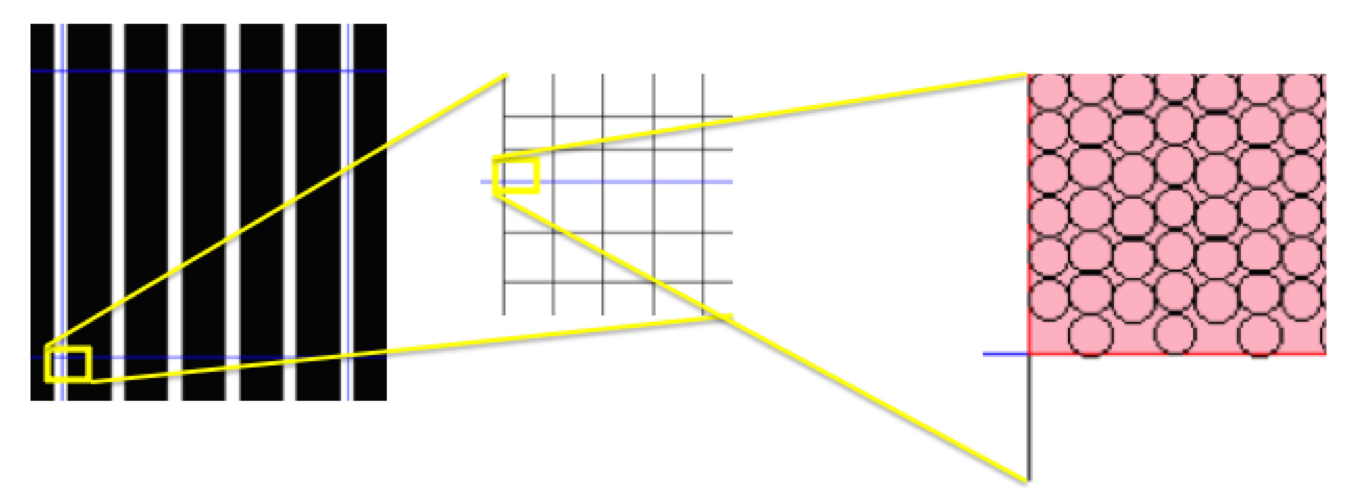
\includegraphics[width=0.8\textwidth]{Field_sizes_cascade_02.png}
   \end{tabular}
  \end{center}
  \caption[CA1a Efficiency]{\label{fig:Hierarchy} Hierarchy of e-beam geometries- in the left panel the grooves are black and the fields are thin blue lines, the middle inset shows subfields, and the right inset shows spots at a regular step spacing.  Spots are the smallest quantum of e-beam dose}
\end{figure}


There are five key geometries in e-beam lithography.  These geometries are probably universal among e-beam tools, though we focus our discussion to the geometries relevant to the JEOL 9300FS.  The geometries, in order of small to large scales are step size, spot size, subfield deflector size, field deflector size, and stage range of motion.  The largest scale geometry- the stage range of motion- simply limits the maximum pattern size, so we do not discuss it in detail in this subsection.  Figure \ref{fig:Hierarchy} shows a cartoon of the hierarchy from left to right- field, subfields, and spots.

\subsubsection{e-beam step size and spot size}
The e-beam step size is the center-to-center separation of the e-beam spots.  In the jackhammer analogy, the step size is the spacing between dithers.  Step sizes can range from 2 to hundreds of nanometers.  We adopted a 50 nm step size for our immersion grating patterns.  The rationale for the step size depends on understanding the e-beam spot size.  

The spot size controls the smallest achievable feature size, as alluded to in Section \ref{sec:Precis}.  Our spot size was between $150-300$ nm, but typically about 230 nm.  Several operational properties of the electron-beam gun affect the spot size, so we mention those here for clarity.  The e-beam gun focuses fast-moving electrons to a spot.  The spot size can be decreased by preferentially removing those electrons with large velocity components perpendicular to the bulk direction of motion.  This preferential removal of fast electrons is achieved with a grounded conductive circular aperture somewhere in the beam path prior to the spot formation.  The aperture is constricted to reduce the spot size.  The net current (e$^-$/s) consequently decreases, since the aperture has effectively thrown away electrons.  So there is a tradeoff between current and spot size.  This tradeoff is important in deciding optimal patterning strategies and sizes.  Our choice of a relatively large spot size ($\sim 200$ nm) came from the economical need to limit the expensive e-beam write time, with the understanding that the spot size is small enough to achieve the specified precision of $< 25$ nm.

The conductive aperture setting coarsely selects the range of spot size achievable.  The detailed spot size depends fine adjustments made to the e-beam column before an exposure.  These adjustments are familiar for those who have used scanning electron microscopy- astigmatism, wobble, and focus, for example.  Poor calibration might deliver an elliptical, asymmetric spot shape.  In practice, a slightly asymmetric spot shape does not affect the performance of immersion gratings.

A key idea is that the step size (50 nm) is much smaller than the spot size ($\sim200$ nm) so that adjacent steps convolve to form a fairly uniform exposure area.  Another key assumption is that the e-beam spot does not change significantly over the course of an exposure.  Our experience is that the e-beam spot is unchanged, so long as the e-beam column is unperturbed.

\subsubsection{Subfield deflector}
The subfield deflector is a component of the e-beam gun that minutely redirects the e-beam spot within a box of up to 4 $\mu$m edge, centered around a mean position.  We selected a $4 \; \mu$m spot for our immersion gratings with coarse grooves ($\sim 27-80 \; \mu$m).  For recent work on fine pitch ($\sim2\; \mu$m) gratings we have experimented with smaller subfield sizes.

\subsubsection{Field deflector}
\label{sec:Field}
The field deflector, also sometimes called the main-field deflector, coarsely redirects the center of the electron beam up to a 500 $\mu$m square.  The main-field deflector can be thought as positioning the center of the subfields.  For example, the choice of a 500 $\mu$m square field size and 4 $\mu$m square field size would result in 125 $\times$ 125 subfields.

The fields are stepped together by the interferometrically controlled stage.  Once an entire field's pattern has been written, the stage steps to the next adjacent field to write.  The stage move speed is typically much slower than the field and subfield deflector speed, so small field sizes are inefficient in time-on-target time compared to wall-clock time.  The performance of the field deflector degrades with distance from the center (e.g. pincushion distortion), so there is a tradeoff between write speed and performance.  

The choice of field size is multifaceted.  Field size choice is one of the key strategies for mitigation of ghosts.  One important idea is that the field size is only a few times larger than our typical immersion grating groove constants.  We define the ratio, $G$, as the field size, $F$, divided by the groove pitch size, $\sigma$.  For example, let's say we have a field size $F\;=\;500\;\mu$m and a groove constant $\sigma \; =\; 100 \; \mu$m.  Then $G\;=\;5$.  So there will be 5 grooves per field.  The omnipresent field deformations will be rubber stamped into each field, repeating every 5 grooves.  The cyclically varying facet positions manifest as ghosts with G-fold symmetry. We expect $G-1$ inter-order ghosts, separated by a fraction $1/G$ of the inter-order separation.  For the $G\;=\;5$ example, there are 4 inter order ghosts, separated by a fifth of the order angular separation.  In Section \ref{sec:MultipleFields} we describe our strategy for mitigating power by distributing the power into multiple fields.

\subsubsection{Interplay of hierarchy at boundaries and design rules}
\label{sec:Boundaries}
The e-beam geometries must match up at the boundaries.  We learned many subtle design rules unique to high performance immersion gratings.  In this subsection we motivate and explain the design rules.

The subfield size must be an integer number of steps.  For example, our choice of subfield size of $4 \; \mu$m has 80 steps of 50 nm each.  The reason for this requirement is that a fractional step is not possible, so the line-edge of contiguous spots would lack a solitary spot near the subfield boundary.  Such a periodic dearth in exposure would manifest as a periodic facet position error along the length of a groove.  The detailed impact on optical phase depends on the relative step size, resist sensitivity, and sundry subsequent processing steps.  Rather than risk a performance degradation it is best practice to avoid the formation of subfield blips in the first place.  

\subsection{Predicting the ghost level associated with field positioning errors}
\label{sec:Ghosts}
\subsection{Employ multiple fields sizes rather than one field size}
\label{sec:MultipleFields}
\subsection{Is there a need for multiple cross-dispersion field sizes?}
\section{Strategies for mitigating facet position errors attributable to large scale stage drift}
\subsection{Characterization of e-beam stage drift}
\subsection{Improvement in wavefront performance from drift correction}
\section{Limitations of direct writing Si immersion gratings}
\subsection{Serial write process yields long write times}
\subsection{Experiments with negative resist}
\subsection{Large per-part investment cost yields heightened process risk}
\section{Conclusions}




\bibliography{SPIE_2014_ebeam}   %>>>> bibliography data in report.bib
\bibliographystyle{spiebib}   %>>>> makes bibtex use spiebib.bst

\end{document} 
